% ============================================================
%  AIAS+ 2026 (Chen Institute Symposium for AI Advancing Science)
%  Full research paper track (6-8 pages), EasyChair Epic Series format.
%  Anonymized for review (CFP enforces an anonymity requirement).
%  References: natbib + apalike (Chicago-family author-date), the
%  build-tested option for easychair.cls (chicago.sty conflicts with
%  the class's thebibliography; biblatex-chicago needs biber).
%  House rule: no em dashes anywhere, including comments.
% ============================================================
\documentclass[letterpaper,withtimes]{easychair}

% --- Math (the class already loads amsthm + empheq, which pulls amsmath) ---
\usepackage{amsmath}     % explicit, no options (avoids empheq option clash)
\usepackage{amssymb}     % class loads latexsym, not amssymb
\usepackage{mathtools}

% --- Tables, floats, spacing helpers ---
\usepackage{booktabs}
\usepackage{xspace}
\usepackage{enumitem}

% --- References: Chicago-family author-date, build-safe with easychair.cls ---
\usepackage[round,authoryear]{natbib}
\setlength{\bibsep}{0pt plus 0.5pt}

% --- Heading spacing (easychair uses standard article sections) ---
\usepackage{titlesec}
\titlespacing*{\section}{0pt}{4pt plus 1pt minus 1pt}{2pt plus 1pt minus 1pt}
\titlespacing*{\subsection}{0pt}{3pt plus 1pt minus 1pt}{1pt plus 1pt minus 1pt}
\titlespacing*{\paragraph}{0pt}{2pt plus 1pt minus 1pt}{0.6em}

% --- Cross-referencing: cleveref LAST (hyperref already loaded by the class) ---
\usepackage[capitalize,noabbrev]{cleveref}

% Do NOT load: hyperref, graphicx, xcolor, geometry, fancyhdr, listings,
% empheq, latexsym, footmisc, mathptmx (the class already loads these).

% ==== Macro kit (ported from the PC-RF source) ====
\newcommand{\grad}{\nabla}
\newcommand{\E}{\mathbb{E}}
\newcommand{\Ea}[1]{\E\left[#1\right]}
\newcommand{\Eb}[2]{\E_{#1}\!\left[#2\right]}
\newcommand{\R}{\mathbb{R}}
\newcommand{\norm}[1]{\left\|#1\right\|}
\newcommand{\proj}{\Pi}
\newcommand{\bI}{\mathbf{I}}
\newcommand{\bc}{\mathbf{c}}
\newcommand{\be}{\mathbf{e}}
\newcommand{\bs}{\mathbf{s}}
\newcommand{\bu}{\mathbf{u}}
\newcommand{\bv}{\mathbf{v}}
\newcommand{\bx}{\mathbf{x}}
\newcommand{\bmu}{{\boldsymbol{\mu}}}
\newcommand{\bphi}{{\boldsymbol{\phi}}}
\newcommand{\pcrf}{\textsc{PC-RF}\xspace}
\newcommand{\etal}{\textit{et al.}\xspace}

% Dense layout: tighten float, display, and caption spacing (no font/margin change).
\setlength{\textfloatsep}{4pt plus 2pt minus 2pt}
\setlength{\intextsep}{4pt plus 2pt minus 2pt}
\setlength{\abovedisplayskip}{3pt plus 1pt minus 1pt}
\setlength{\belowdisplayskip}{3pt plus 1pt minus 1pt}
\setlength{\abovedisplayshortskip}{1.5pt plus 1pt}
\setlength{\belowdisplayshortskip}{1.5pt plus 1pt}
\setlength{\abovecaptionskip}{2pt}
\setlength{\belowcaptionskip}{0pt}

\title{Physics-Constrained Rectified Flow for\\ Climate Downscaling}

% Anonymized for review (AIAS+ anonymity requirement).
\author{Anonymous Author(s)}
\institute{Anonymous Institution}
\authorrunning{Anonymous}
\titlerunning{Physics-Constrained Rectified Flow for Climate Downscaling}

\begin{document}
\maketitle

\begin{abstract}
Statistical downscaling turns a coarse climate projection or reanalysis product into a high-resolution regional field, recovering the mesoscale structure, convective rain bands, orographic enhancement, and sharp wind gradients, behind local impacts such as flooding and crop stress. The problem carries direct stakes for adaptation and resilience, yet many methods struggle to preserve fine-scale spatial dependencies, and modern diffusion and flow-matching generators can produce sharp fields that still violate the atmospheric conservation laws encoded in their coarse conditioning. We present Physics-Constrained Rectified Flow (\pcrf), a conditional flow-matching downscaler that enforces physical consistency in both training and inference. During training, three differentiable penalties act on a one-step clean-field estimate: a divergence-free constraint on wind, a non-negativity penalty on precipitation, and a mass-conservation term coupling each fine field to its coarse integral. At inference, a projection makes non-negativity and domain mass balance hold exactly. On a controlled synthetic benchmark that isolates the constraint mechanism, \pcrf drives the non-negativity violation rate and mass-conservation error of an unconstrained baseline (0.236 and 0.184) to exactly zero while improving reconstruction (RMSE 0.140 to 0.112, SSIM 0.52 to 0.68) and lowering divergence error by about 30\%, evidence that the penalties act as inductive structure rather than a fidelity tax. On a real single-year ERA5 task, the inference projection secures exact validity for both the constrained and unconstrained models, and \pcrf retains a small perceptual edge (SSIM 0.914 vs.\ 0.912, PSNR 26.59 vs.\ 26.39, CRPS 1.149 vs.\ 1.188). We propose three physics-validity metrics, Divergence Error, Non-negativity Violation Rate, and Mass-Conservation Error, for the standard evaluation suite of generative climate downscaling.
\end{abstract}

\noindent\textbf{Keywords:} Climate Downscaling, Physics-Constrained Generative Models, Rectified Flow, Diffusion Models, Conservation Laws, AI for Science.

\section{Introduction}
\label{sec:intro}
Given coarse-resolution projections from global climate models or satellite products, statistical downscaling estimates a high-resolution regional field, putting back the sub-grid texture and local contrasts of a target variable such as precipitation, near-surface wind, or sea level. It does this by learning a statistical relationship between coarse inputs and high-resolution historical observations, and the detail it recovers is what adaptation runs on, since the harms of a warming climate land at local scales that a coarse grid never represents. \Cref{fig:motivation} makes the resolution gap visible with a sea surface height anomaly off the Ecuador and Peru coast (12 August and 3 October 2023); the coarse altimetric background keeps only the broad gradient, while the red boxes mark the mesoscale structure that downscaling must restore (\pcrf downscales atmospheric fields; the example only makes the resolution gap visible), adapted from prior downscaling work. \Cref{fig:pipeline} shows the corresponding coarse-to-fine pipeline. We work with reanalysis, where ERA5~\citep{hersbach2020era5} resolves only 0.25\textdegree\ (about 25\,km at mid-latitudes), too coarse for the sub-kilometer variability behind flooding and coastal inundation.

The stakes are concrete. Global models project harms that run from extreme weather to higher seas and lost crop yield, and none of them arrives on the model's own coarse grid. A small shift in regional conditions is what floods a coastal town or pushes a growing season past the heat it can bear, while a water manager sizing a reservoir, or a planner siting a wind farm, needs conditions at the basin scale rather than a continental average. Coastal regions show the stakes most sharply, since with sea-level rise even a small change drives flooding, erosion, and habitat loss~\citep{IPCC2021, Rabinowitz2023}, and the high-resolution fields that resolve such risk are what coastal management and disaster preparedness depend on. Downscaling delivers these risks at the scale where adaptation and mitigation are actually decided.

\begin{figure}[t]
\centering
\includegraphics[width=0.55\linewidth]{figures/motivation_kriging.png}
\caption{Resolution gap, sea surface height anomaly.}
\label{fig:motivation}
\end{figure}

\begin{figure}[t]
\centering
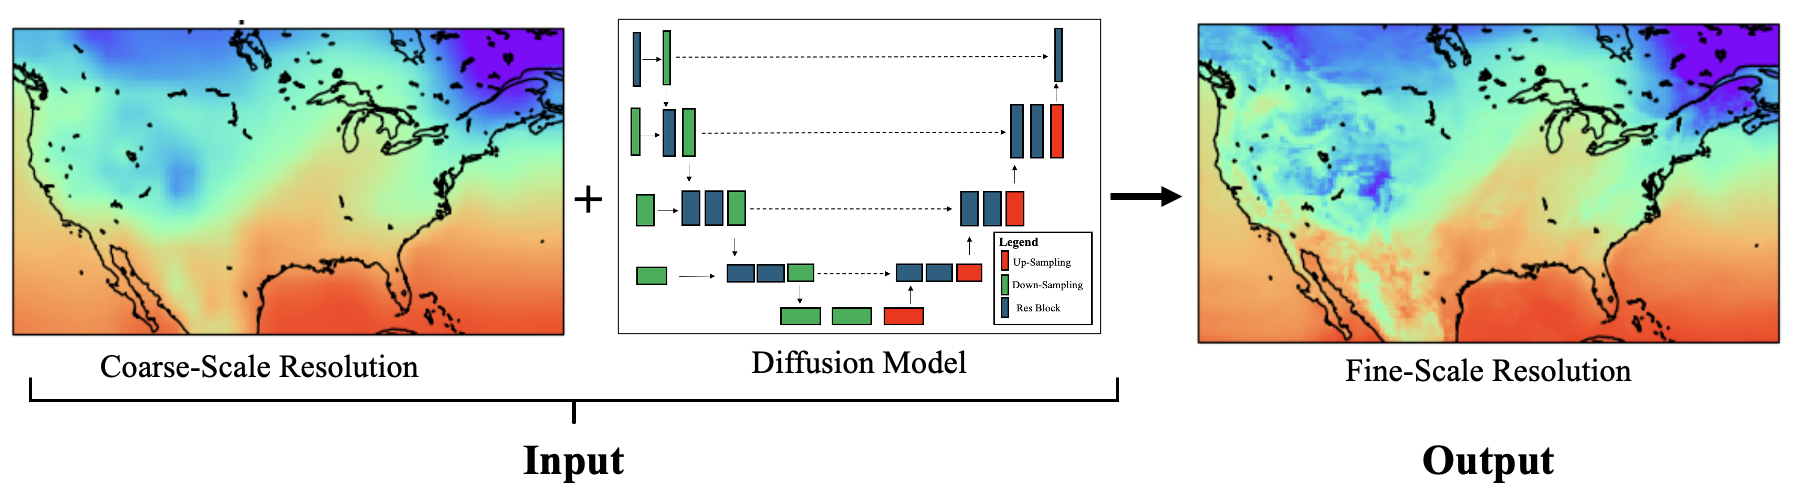
\includegraphics[width=0.90\linewidth]{figures/motivation.png}
\caption{The coarse-to-fine downscaling pipeline. A coarse, low-resolution input field (left) is passed, together with its conditioning context, through the generative model (center) to a high-resolution output field (right) that restores the fine-scale structure the coarse input averages away. The example maps show a near-surface temperature field over North America, where the downscaled output resolves regional contrasts absent from the input.}
\label{fig:pipeline}
\end{figure}

Two properties make the task hard. A climate field ties spatial and temporal dependence together under several drivers acting at once. Atmospheric circulation, orographic forcing, the contrast between convective and stratiform precipitation, and synoptic weather all leave their mark on the same field. The field is also non-stationary, so as circulation regimes drift and extremes hit, even its mean and spread move over time, and a model fit to one stretch of years carries no promise of holding in the next. Recovering a fine field from a coarse one is also ill-posed. The fine state must be backed out from a forward model and sparse coarse observations, and nonlinear coupling with model uncertainty leaves the answer non-unique, calling for a method that is both physically grounded and probabilistic.

The past few years have seen a rapid shift toward deep generative downscaling. Diffusion models such as CorrDiff~\citep{mardani2023residual} and ensemble diffusion approaches~\citep{price2023gencast} produce spatially coherent, high-fidelity precipitation and wind at unprecedented resolution, while global data-driven forecasters such as GraphCast~\citep{lam2023graphcast} have reshaped medium-range prediction. Rectified flow~\citep{liu2022flow,lipman2022flow}, which straightens generative trajectories from noise to data, can sample in far fewer neural function evaluations at competitive quality, an important property at downscaling resolutions. Borrowing a natural-image super-resolution network wholesale works less well. A network of that kind imposes no physics and ignores the nonlinear interactions that tie parts of the Earth system together, and in its deterministic form it hands back a single point estimate with none of the uncertainty climate forecasting needs. A purely pixel-wise or perceptual objective also gives no guarantee that the output respects the atmospheric physics carried in its coarse conditioning. Generated wind can diverge, precipitation go negative, and domain mass drift from the coarse input.

Physics-informed neural networks~\citep{raissi2019physics} embed PDE residuals as soft constraints for regression, and physics penalties have appeared in fluid simulation~\citep{kochkov2021machine} and molecular generation~\citep{kohler2020equivariant}, yet their use inside flow-matching models for atmospheric downscaling stays underexplored. Prior work~\citep{sharma2024kriging} embedded geostatistical priors in conditional diffusion for sea-level downscaling, and \pcrf carries that line to rectified flow and to atmospheric conservation laws. Physical validity here splits into two separable claims. Training penalties shape the generated field, and an inference-time projection makes it valid by construction.

\noindent\textbf{Contributions:} We make three contributions.
\begin{itemize}[noitemsep,topsep=0pt]
\item We propose Physics-Constrained Rectified Flow (\pcrf), a conditional rectified-flow downscaler that enforces divergence-free wind, non-negative precipitation, and domain mass conservation through differentiable penalties, paired with an inference-time projection that makes the hard constraints exact.
\item We introduce three physics-validity metrics, Divergence Error (DE), Non-negativity Violation Rate (NVR), and Mass-Conservation Error (MCE), as complements to SSIM, PSNR, and CRPS for generative climate downscaling.
\item We separate training from inference effects on synthetic and real ERA5 data, showing that the projection guarantees validity for both models while the penalties account for the perceptual and synthetic-divergence gains.
\end{itemize}

\section{Diffusion and Flow Matching}
\label{sec:background}
Conditional generative downscaling treats the fine field as a sample from a distribution conditioned on the coarse field. Denoising diffusion models~\citep{ho2020denoising,song2021score} define a forward process that gradually corrupts a clean field $\bx_0$ into Gaussian noise,
\begin{equation}
q(\bx_t \mid \bx_0) = \mathcal{N}\!\left(\bx_t;\ \sqrt{\psi_t}\,\bx_0,\ (1-\psi_t)\,\bI\right), \qquad \psi_t = \prod\nolimits_{i=1}^{t}\alpha_i,
\label{eq:fwd}
\end{equation}
with a per-step schedule $\alpha_t \in (0,1)$, and learn a reverse chain that denoises back to data conditioned on a context $\bc$,
\begin{equation}
p_\theta(\bx_{t-1} \mid \bx_t, \bc) = \mathcal{N}\!\left(\bx_{t-1};\ \bmu_\theta(\bx_t, t, \bc),\ \sigma_t^2\,\bI\right).
\label{eq:rev}
\end{equation}
Sampling from~\labelcref{eq:rev} requires hundreds to thousands of network evaluations along a stochastic chain. Rectified flow~\citep{liu2022flow,lipman2022flow} replaces this stochastic reverse process with a deterministic transport along straight paths from noise to data, which we adopt for its sampling efficiency at the high spatial resolutions of downscaling.

\paragraph{Rectified flow:}
Rectified flow learns a velocity field $\bv_\theta$ that transports samples from a source $p_0$ (Gaussian) to a target $p_1$ (data) along straight trajectories. Given paired samples $(\bx_0,\bx_1)$, the linear interpolation $\bx_t = (1-t)\bx_0 + t\bx_1$ induces the objective
\begin{equation}
\mathcal{L}_{\mathrm{RF}} = \Eb{t, \bx_0, \bx_1}{ \norm{ \bv_\theta(\bx_t, t, \bc) - (\bx_1 - \bx_0) }_2^2 },
\label{eq:rf}
\end{equation}
where $\bc$ is the conditioning context. Inference integrates the ODE $d\bx_t/dt = \bv_\theta(\bx_t, t, \bc)$ from $t{=}0$ to $t{=}1$ with an Euler or Runge--Kutta solver in 10--20 steps. The straightened trajectories permit far fewer evaluations than the stochastic chain of~\labelcref{eq:rev}.

\paragraph{Problem formulation:}
Let $\bx_c \in \R^{H_c \times W_c \times C}$ be a coarse climate field (ERA5 precipitation and $u$/$v$ wind at 0.25\textdegree) and $\bx_f \in \R^{H_f \times W_f \times C}$ the fine target at upscaling factor $r$, so $H_f = r H_c$ and $W_f = r W_c$. An optional satellite observation $\bs$ supplies land-surface context. We train $\bv_\theta(\bx_t, t, \bc)$ conditioned on $\bc = (\bx_c^{\uparrow}, \bphi(\bs))$, where $\bx_c^{\uparrow}$ is the bicubically upsampled coarse field and $\bphi(\bs)$ is an encoded land-surface embedding (described below).

\paragraph{Physics penalties:}
We augment~\labelcref{eq:rf} with three differentiable penalties evaluated on the one-step clean-field estimate $\hat\bx_f = \bx_t + (1-t)\,\bv_\theta(\bx_t, t, \bc)$. For horizontal wind $(\hat u, \hat v)$, incompressibility requires $\grad\cdot\hat\bu = 0$, penalized as
\begin{equation}
\mathcal{L}_{\mathrm{div}} = \Ea{ \norm{ \tfrac{\partial \hat u}{\partial x} + \tfrac{\partial \hat v}{\partial y} }_2^2 },
\label{eq:div}
\end{equation}
with derivatives by central finite differences. Precipitation is non-negative, so we penalize $\mathcal{L}_{\mathrm{nn}} = \Ea{\norm{\min(\hat p, 0)}_2^2}$. The fine-resolution precipitation integral should match the coarse total, preventing the generator from adding or removing precipitation at the domain scale.
\begin{equation}
\mathcal{L}_{\mathrm{mass}} = \Ea{ \left| \tfrac{1}{H_f W_f}\textstyle\sum_{i,j} \hat p_{ij} - \tfrac{1}{H_c W_c}\textstyle\sum_{i',j'} p^c_{i'j'} \right|^2 }.
\label{eq:mass}
\end{equation}
The full loss combines the flow objective with the penalties, $\mathcal{L} = \mathcal{L}_{\mathrm{RF}} + \lambda_1 \mathcal{L}_{\mathrm{div}} + \lambda_2 \mathcal{L}_{\mathrm{nn}} + \lambda_3 \mathcal{L}_{\mathrm{mass}}$, with $\lambda_i$ set on validation.

\paragraph{Why these constraints:}
The three penalties are not generic regularizers. They encode atmospheric physics that a downscaled field must respect to be usable downstream. Horizontal wind on synoptic scales is nearly incompressible, so a non-zero divergence signals spurious sources or sinks of air that no physical flow would produce. Precipitation is a non-negative accumulation, so a negative value is a physical impossibility that breaks any hydrological model fed the field. Domain mass balance ties the fine precipitation total to the coarse input, which prevents the generator from inventing or destroying water at the regional scale, the quantity that basin-scale runoff and flood models integrate. A field that violates these laws can score well on perceptual metrics while remaining unusable for physical inference, which is why we measure validity directly.

\paragraph{Inference-time projection:}
The penalties encourage validity but do not enforce it. After integrating the sampling ODE we apply a projection $\proj$, where a softplus rectification maps precipitation to non-negative values and a multiplicative rescaling restores the coarse mass exactly,
\begin{equation}
\hat\bx_f \;\leftarrow\; \proj\!\left( \hat\bx_f \,;\, \bx_c \right).
\label{eq:proj}
\end{equation}
\Cref{eq:proj} makes NVR and MCE exactly zero at inference time for any model, independent of whether the penalties were used. In practice \pcrf combines the two effects. The penalties shape the field, and the projection guarantees the hard constraints.

\paragraph{Land-surface conditioning:}
To couple atmospheric state with the land surface, \pcrf admits a conditioning path over Sentinel-2 Level-2A imagery~\citep{drusch2012sentinel}, co-registered to the target grid. A ResNet encoder $\bphi$ maps three vegetation and moisture indices (NDVI, NDWI, SAVI) and the stacked bands to an embedding, fused with the coarse conditioning through feature-wise linear modulation~\citep{perez2018film}. The architecture supports this path, and its empirical evaluation is ongoing, so we report no Sentinel-2 results here.

\paragraph{Architecture:}
The velocity network $\bv_\theta$ is a U-Net~\citep{ronneberger2015unet} with sinusoidal time embedding and cross-attention at each resolution, skip connections from encoder to decoder, and the land-surface conditioning injected through FiLM. The trained model has 7.6M parameters, small by design. \Cref{fig:arch} summarizes the pipeline.

\begin{figure}[t]
\centering
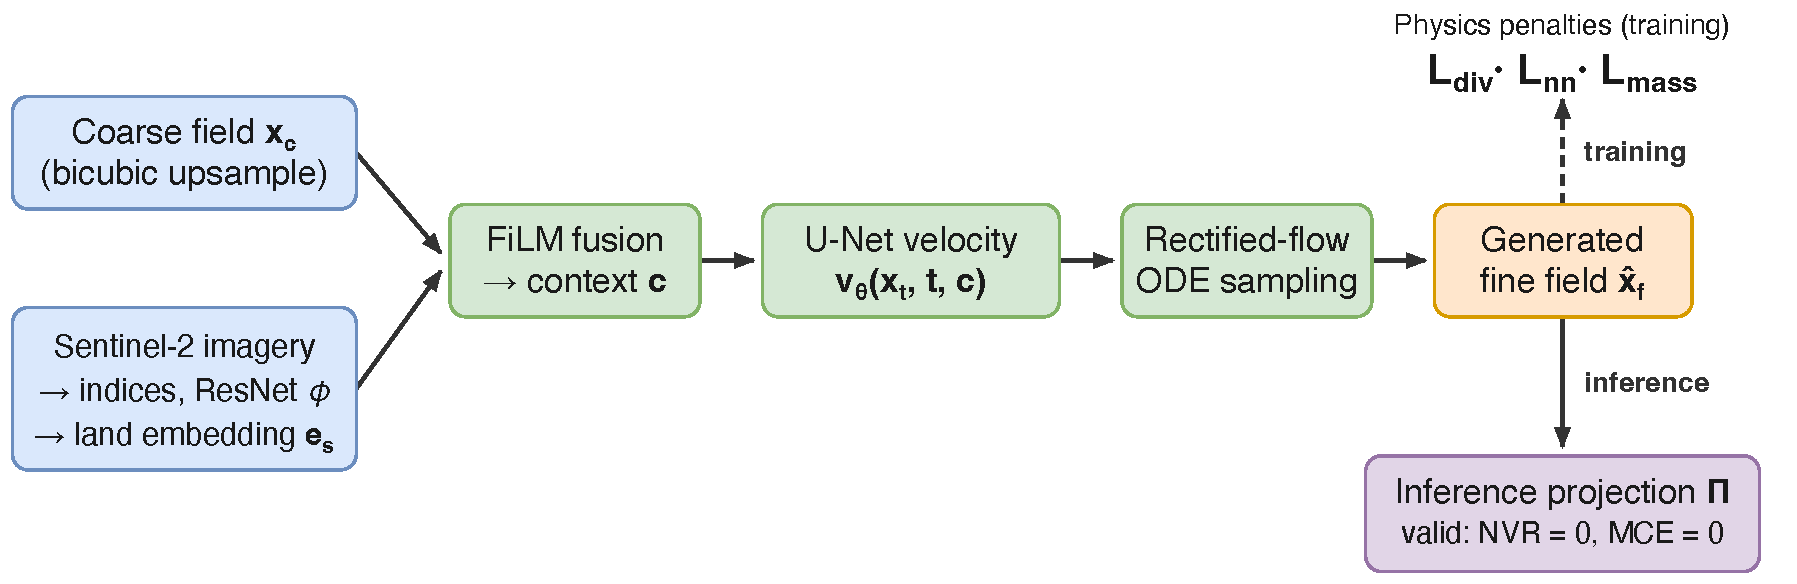
\includegraphics[width=\linewidth]{figures/architecture.pdf}
\caption{The \pcrf framework. The coarse climate field $\bx_c$ is upsampled to provide atmospheric conditioning, and Sentinel-2 imagery is reduced to spectral indices and encoded into a land-surface embedding. The two paths are fused by FiLM into a context $\bc$ that conditions the U-Net velocity field $\bv_\theta(\bx_t, t, \bc)$. Sampling integrates the rectified-flow ODE to produce $\hat\bx_f$, on which the divergence-free, non-negativity, and mass-conservation penalties are evaluated, and the inference projection $\proj$ then makes non-negativity and mass balance exact.}
\label{fig:arch}
\end{figure}

\section{Experiments}
\label{sec:experiments}
We ask whether physics constraints reduce physical-law violations without degrading perceptual quality, and we separate the effect of the training penalties from that of the inference projection. We report SSIM, PSNR, and probabilistic CRPS alongside three physics-validity metrics. Divergence Error (DE) is the mean $|\grad\cdot\hat\bu|$ over the test set. Non-negativity Violation Rate (NVR) is the fraction of precipitation cells with $\hat p < 0$. Mass-Conservation Error (MCE) is the relative error between domain-integrated fine precipitation and the coarse input.

\noindent\textbf{Experiment Setup:}
The real-data task uses ERA5 hourly total precipitation and 10\,m $u$/$v$ wind at 0.25\textdegree~\citep{hersbach2020era5} for 2020. ERA5 is the ECMWF fifth-generation reanalysis, which assimilates surface and satellite observations into a physically consistent global record, so the coarse and fine fields share one dynamical basis and the conservation diagnostics below are physically meaningful. It contains 1171 training samples, roughly 36 optimization steps per epoch, with a held-out temporal split for validation and test. The model downscales by a fixed integer factor $r$. The velocity network is the 7.6M-parameter U-Net described in \cref{sec:background}. We train with AdamW for 300 epochs at batch size 32, learning rate in $[10^{-4}, 5{\times}10^{-4}]$, and physics weights $\lambda_1{=}\lambda_2{=}\lambda_3{=}1.0$ for the reported runs. The main run uses one NVIDIA A100-40GB at about 74.6\,s/epoch; the main run plus ablations total roughly 21 A100 GPU-hours. All penalties are computed on the one-step clean-field estimate $\hat\bx_f$. The reference implementation is modular PyTorch with 46 CPU unit tests and an end-to-end test asserting the projection drives NVR to $0$ and MCE below $10^{-3}$; the velocity field exports to ONNX for deployment.

\paragraph{Synthetic Mechanism Check:}
Before reporting on real reanalysis, we isolate the constraint mechanism on a controlled synthetic task whose ground truth is physically exact by construction (divergence-free wind from a stream function, non-negative precipitation from Gaussian blobs, a known coarse mass), isolating the constraint pathway from reanalysis confounds. \Cref{tab:synthetic} compares an unconstrained baseline (RF-base, the truth plus correlated noise and a negative bias) to \pcrf. Relative to RF-base, \pcrf lowers divergence error by about 30\% ($0.0081\to0.0057$), removes all non-negativity violations (NVR $0.236\to0$), drives mass-conservation error to zero, and improves fidelity (correlation $0.956\to0.966$, SSIM $0.518\to0.682$). The synthetic results isolate and confirm the constraint pathway, and we keep them distinct from the real-data ERA5 results below.

\begin{table}[t]
\caption{Synthetic mechanism check (pure numpy, fixed seed). \emph{Not} ERA5 results. $\uparrow$ higher is better, $\downarrow$ lower is better.}
\label{tab:synthetic}
\centering
\small
\begin{tabular}{lcccccc}
\toprule
\textbf{Method} & DE$\downarrow$ & NVR$\downarrow$ & MCE$\downarrow$ & RMSE$\downarrow$ & Corr$\uparrow$ & SSIM$\uparrow$ \\
\midrule
Ground truth & 0.0000 & 0.000 & 0.0000 & 0.0000 & 1.000 & 1.000 \\
RF-base (no physics) & 0.0081 & 0.236 & 0.1838 & 0.1397 & 0.956 & 0.518 \\
\textbf{\pcrf (physics)} & \textbf{0.0057} & \textbf{0.000} & \textbf{0.0000} & \textbf{0.1116} & \textbf{0.966} & \textbf{0.682} \\
\bottomrule
\end{tabular}

\end{table}

\paragraph{Real ERA5 Downscaling:}
We next evaluate on the single-year ERA5 precipitation downscaling task. \Cref{tab:era5} compares \pcrf against the unconstrained RF-base. A broader baseline suite (bicubic, SRCNN, SRGAN, a DDPM downscaler, and CorrDiff) is still running and we report it in future work rather than with placeholder numbers here. The inference projection drives NVR and MCE to exactly zero for both models, so on real data physical validity is guaranteed by construction. Physically, the divergence penalty suppresses spurious convergence that would imply nonphysical vertical motion, and the mass term keeps the regional water budget closed, the quantity basin-scale runoff and flood models integrate. \pcrf also retains a perceptual edge over RF-base (SSIM $0.912\to0.914$, PSNR $26.39\to26.59$, CRPS $1.188\to1.149$), consistent with the synthetic finding that the penalties shape the field at no fidelity cost.

\begin{table}[t]
\caption{Real single-year ERA5 precipitation downscaling (one A100). NVR and MCE are exactly zero for both models because the inference projection enforces them. A broader baseline comparison is deferred to future work. Best in \textbf{bold}. $\uparrow$ higher is better, $\downarrow$ lower is better.}
\label{tab:era5}
\centering
\small
\begin{tabular}{lccccc}
\toprule
\textbf{Method} & SSIM$\uparrow$ & PSNR$\uparrow$ & CRPS$\downarrow$ & NVR$\downarrow$ & MCE$\downarrow$ \\
\midrule
RF-base & 0.912 & 26.39 & 1.188 & 0.000 & 0.0000 \\
\textbf{PC-RF} & \textbf{0.914} & \textbf{26.59} & \textbf{1.149} & \textbf{0.000} & \textbf{0.0000} \\
\bottomrule
\end{tabular}

\end{table}

\paragraph{Ablation:}
\Cref{tab:ablation} removes one physics penalty at a time on the real ERA5 task. Two patterns hold. First, NVR and MCE are exactly zero in every row, including RF-base, because the projection enforces them after sampling. Second, the divergence penalty is the one with a measurable training effect. Removing it raises Divergence Error (full $0.0634$ to $0.0649$), the expected direction, while removing the non-negativity or mass penalty leaves DE and SSIM within run-to-run noise (SSIM $0.912$ to $0.915$ across all arms). On real data the penalties therefore do not degrade perceptual quality, and the largest separation between constrained and unconstrained models appears in the controlled synthetic setting.

\begin{table}[t]
\caption{Ablation on real ERA5, a separate training run from the headline ERA5 comparison. Each row removes one physics penalty. NVR and MCE are exactly zero for every arm.}
\label{tab:ablation}
\centering
\small
\begin{tabular}{lcccc}
\toprule
\textbf{Configuration} & SSIM$\uparrow$ & DE$\downarrow$ & NVR$\downarrow$ & MCE$\downarrow$ \\
\midrule
Full \pcrf                  & 0.912 & \textbf{0.0634} & 0.000 & 0.0000 \\
$-$ divergence penalty      & 0.912 & 0.0649          & 0.000 & 0.0000 \\
$-$ non-negativity penalty  & 0.913 & 0.0644          & 0.000 & 0.0000 \\
$-$ mass penalty            & 0.915 & 0.0639          & 0.000 & 0.0000 \\
RF-base (no physics)        & 0.913 & 0.0643          & 0.000 & 0.0000 \\
\bottomrule
\end{tabular}
\end{table}

\section{Related Work}
\label{sec:related}
Deep generative models offer several routes from coarse to fine, each with distinct trade-offs for climate downscaling. Generative adversarial networks~\citep{goodfellow2014generative} drove early single-image super-resolution~\citep{ledig2017photo,dong2015image} and were adapted to the geosciences, where adversarial super-resolution recovers fine-scale wind and solar structure~\citep{stengel2020adversarial} and stochastic variants downscale time-evolving atmospheric fields with calibrated spread~\citep{leinonen2021stochastic}, though adversarial training is unstable and offers no explicit likelihood. Normalizing flows~\citep{rezende2015variational,dinh2017density,kingma2018glow} give exact likelihoods through invertible maps and have been applied to unsupervised climate downscaling~\citep{groenke2020climalign}, at the cost of architectural restrictions that limit expressivity at high resolution. Denoising diffusion~\citep{ho2020denoising,song2021score} and the diffusion downscalers CorrDiff and GenCast~\citep{mardani2023residual,price2023gencast} now lead on sample quality and calibration on community benchmarks~\citep{rasp2024weatherbench}, while rectified flow~\citep{liu2022flow,lipman2022flow} retains that quality and straightens the generative path for far cheaper sampling, which is why \pcrf builds on it.

Across these families, physical consistency is usually treated as a diagnostic rather than a built-in constraint, so a model can minimize a perceptual or likelihood objective and still miss the fine-scale spatial correlations that decide whether a downscaled field is physically plausible. Classical statistical downscaling and interpolation~\citep{maraun2018statistical,vandal2017deepsd} capture spatial structure but lean on a stationarity assumption and oversmooth, washing out the fine-scale detail that drives regional risk. Physics-informed learning~\citep{raissi2019physics} and physically-regularized simulation~\citep{kochkov2021machine,kohler2020equivariant} embed governing equations as soft penalties, but mostly for forward modeling rather than conditional generation, and they rarely guarantee the constraint at sampling time. Geostatistics-informed diffusion embeds a spatial prior in a conditional diffusion downscaler for sea level; \pcrf carries that line to rectified flow and to atmospheric conservation laws. \pcrf differs in two ways. It places conservation laws inside a rectified-flow objective for downscaling, and it pairs the soft penalties with a hard inference-time projection, which lets us measure separately what training changes and what inference guarantees.

\section{Conclusion}
\label{sec:conclusion}
In this paper, we introduced a physics-constrained rectified-flow downscaler that enforces divergence-free wind, non-negative precipitation, and mass conservation through differentiable penalties, and that makes the hard constraints exact with an inference-time projection. On a controlled synthetic benchmark the penalties remove all non-negativity and mass-conservation violations while improving reconstruction, and on real single-year ERA5 the projection guarantees validity for both constrained and unconstrained models while \pcrf keeps a small perceptual edge. The practical lesson is that physical validity for generative scientific models is best secured at inference time, with training penalties improving the field that the projection then certifies. Finally, we proposed three physics-validity metrics as standard additions to downscaling benchmarks.

\paragraph{Future work:}
We are completing the broader baseline comparison against bicubic, SRCNN~\citep{dong2015image}, SRGAN~\citep{ledig2017photo}, a DDPM downscaler, and CorrDiff~\citep{mardani2023residual}, and scaling \pcrf to multi-year and global ERA5 across regions, seasons, and extreme events. We are also finishing the Sentinel-2 land-surface evaluation, integrating pretrained Earth-observation encoders, and adding a thermodynamic-consistency penalty.

\paragraph{Broader impact:}
We target scientific decision support, where invalid fields such as negative precipitation or mass drift can mislead hydrological and agricultural models, a risk the projection reduces. Validated on one year of ERA5 and a synthetic benchmark, it should not drive operational forecasting without broader evaluation across regions, seasons, and extremes.

\bibliographystyle{apalike}
{\footnotesize\linespread{0.93}\selectfont \bibliography{refs}}

\end{document}
